\documentclass[10pt]{article}
\usepackage[utf8]{inputenc}
\usepackage{hyperref}
\usepackage{fontenc}
\usepackage{mathptmx}
\usepackage{geometry}
\usepackage{titling}
\usepackage{graphicx}
\usepackage{subcaption}
\usepackage{pdfpages}


\usepackage[noend]{algorithmic}
\newcommand{\TITLE}[1]{\item[#1]}
\renewcommand{\algorithmiccomment}[1]{$/\!/$ \parbox[t]{4.5cm}{\raggedright #1}}
% ugly hack for for/while
\newbox\fixbox
\renewcommand{\algorithmicdo}{\setbox\fixbox\hbox{\ {} }\hskip-\wd\fixbox}


\setlength{\topskip}{0mm}
\setlength{\droptitle}{-8em} 
\title{{\large \textbf{CONCORDIA UNIVERSITY \\ DEPARTMENT OF COMPUTER SCIENCE AND SOFTWARE ENGINEERING \\ SOEN 6011: SOFTWARE ENGINEERING PROCESSES \\ SECTION CC WINTER 2019 \\ F1: $arccos(x)$}  \\ Changes from $D_2$ to $D_3$: Section 5 \& 6 }}
\author{\normalsize \textbf {STUDENT NAME: YONGCONG LEI} \\ \normalsize \textbf{STUDENT IDENTIFICATION NUMBER: 40045701} \\ \normalsize \textbf{GITHUB REPOSITORY: https://github.com/WingCuengRay/SOEN6011\_Summer19}}
\date{}
\begin{document}
\maketitle

\section{Characteristics and Domain}
\subsection{Characteristics}

\begin{enumerate}
    \item $arccos(x)$ is an inverse trigonometric function (relate an angle of a right-angled triangle to ratios of two side lengths), and it's tightly related to the trigonometric cosine function.
    
    \begin{figure}[h!]
      \centering
      \begin{subfigure}[b]{0.4\linewidth}
        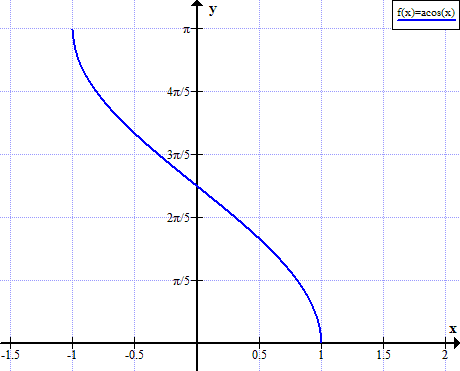
\includegraphics[width=\linewidth]{image/arccos.png}
        \caption{$arccos(x)$}
      \end{subfigure}
      \begin{subfigure}[b]{0.4\linewidth}
        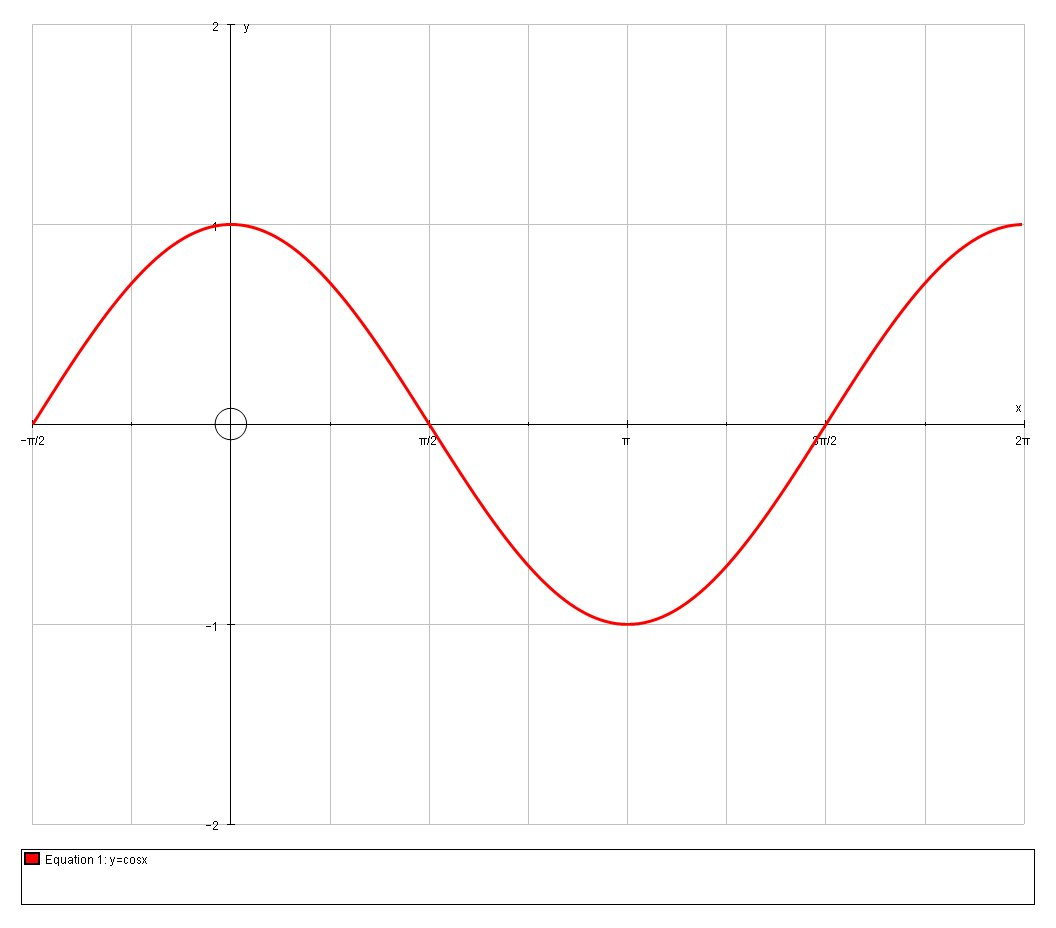
\includegraphics[width=\linewidth]{image/cos.jpg}
        \caption{$cos(x)$}
      \end{subfigure}
      \caption{$arccos(x)$ and $cos(x)$}
      \label{fig:coffee}
    \end{figure}

    
    \item $arccos(x)$ is an inverse trigonometric functions of $cos(x)$. In order introduce inverse trigonometric functions, we first need to take a look at trigonometric functions. In mathematics, the trigonometric functions are real functions which relate an angle of a right-angled triangle to ratios of two side lengths\cite{einstein}. $cos(x)$ is one of them. Given $$x = cos(y) = \frac{b}{h} = \frac{adjacent}{hypotenuse}$$ then $$y = arccos(x)$$ Figure 1 is an example of $cos(x)$. In this case, $x = cos(y) = \frac{OC}{OA}$. Therefore, $y = arccos(x) = arccos(\frac{OC}{OA})$.
    \begin{center}
      \begin{figure}[h!]
          \centering
          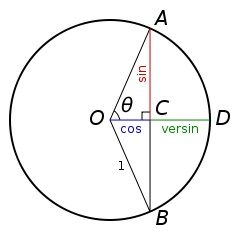
\includegraphics[width=0.3\linewidth]{image/cos_detail.jpg}
          \caption{trigonometric functions}
          \label{fig:my_label}
      \end{figure}
    \end{center}
    
    \item The function $arccos$ has their \textbf{principle values}. It's because inverse cosine function are not one-to-one.Therefore, the ranges of the inverse cosine functions are proper subsets of the domains of the original functions. With this restriction, for each x in the domain the expression $arccos$ will evaluate only to a single value, called its principal value. The range of principle values of $arccos(x)$ is $[-\frac{1}{2}\pi, \frac{1}{2}\pi]$. As a result, there will be one-to-one relationship for any value in domain.
\end{enumerate}

\subsection{Domain and Co-domain}
\paragraph{}
Since none of the six trigonometric functions are one-to-one, they are restricted in order to have inverse functions. The co-domain of $arccos(x)$ in area $[-\infty, \infty]$. However, we usually takes the principle values as its co-domain which is $[-\frac{1}{2}\pi, \frac{1}{2}\pi]$. Therefore, there will be one-to-one relationship between its domain and co-domain.

\paragraph{}
As a result, the domain is $x \in [-1, 1]$. The co-domain is $y \in [-\frac{1}{2}\pi, \frac{1}{2}\pi]$ for the equation $y = arccos(x)$.

\pagebreak
\section{Requirements}
\begin{enumerate}
    \item When a user apply a value $x \in [-1, 1]$ (which is the domain) to function $arccos(x)$, the calculator shall return a value $y\in [0, \pi]$.
    \item When a user apply a value $x \notin [-1, 1]$, the calculator shall show an error message.
    \item If the result is a infinite decimal, the result shall be shown to the nearest five decimal points.
    \item The calculator shall support input of operands such as digits or special irrational number such as $\pi, e$ etc.
    \item When a user enter anything to the calculator, the calculator shall show anything that user input.
    \item When a user input an invalid sequence of operands and operators, a error message shall be shown.
    \item When a user reset the calculator, all the ongoing transaction and history should be erased.
    \item The user shall be able to correct or modify his input to the calculator.
    \item The calculator shall be able to save the input sequence and related result to its memory.
\end{enumerate}

\pagebreak
\section{Algorithms}
\begin{enumerate}
    \item The algorithm uses the Lagrange Polynomial Approximation to calculate the arccos(x). The advantage of the algorithm is its performance. The time complexity is constant time. The advantage is that it has a maximum error of about 0.18 rad. Besides, The polynomial approximation performs pretty bad near $x=-1$ or $x=1$ where the derivative of the inverse cosine goes to infinity. Here is the pseudocode of the algorithhm. \newline
    
    \begin{algorithmic}[1]
      \TITLE{\textsc{Lagrange-polynomial-Approximation-arccos}$(x)$}
      \STATE $x\_square = x*x$
      \STATE $v1 = -0.69813170079773212 * x\_square - 0.87266462599716477$
      \STATE return $v1 * x + 1.5707963267948966$
    \end{algorithmic}

    \item Besides, there is an algorithm for $arccos(x)$ based on rational function - the quotient of two polynomials. The advantage is that it can give a a much better approximation. It has a maximum absolute error of 0.017 radians (0.96 degrees) on the interval (-1, 1). The disadvantage of the algorithm is that it involves division operator. In some cases, division is more expensive than addition and multiplication. Here is the pseudocode of the algorithm. \newline
    
    \begin{algorithmic}[1]
      \TITLE{\textsc{rational-function-Approximation-arccos}$(x)$}
      \STATE $a = -0.939115566365855$
      \STATE $b =  0.9217841528914573$
      \STATE $c = -1.2845906244690837$
      \STATE $d =  0.295624144969963174$
      \STATE $x\_square = x*x$
      \STATE $x\_cube = x\_square*x$
      \STATE $x\_quad = x\_cube*x$;
      \STATE return $(\pi / 2 + (a*x + b*x\_cube) / (1+ c*x\_square + d*x\_quad) )$
    \end{algorithmic}
\end{enumerate}

\pagebreak
\section{Problem 4}
\subsection{Debugger}
\subsubsection{Description}
\paragraph{}
I choose the debugger tools in IntelliJ IDEA as the debugger of my application. It provides a full range of facilities of debugging in source code, including but no limitting: 
\begin{enumerate}
    \item Breakpoints in Java.
    \item Customizable breakpoint properties: conditions, pass count, and so on.
    \item Frames, variables, and watches views in the debugger UI.
    \item Runtime evaluation of expressions.
\end{enumerate}

\subsubsection{Advantage}
\paragraph{}
There are lots of \textbf{advantages} with the debugging tool set in IntelliJ IDEA. 

\begin{enumerate}
    \item It provides a simple but powerful user interface for debugging. User can easy create various kinds of breakpoints, such as conditional breakpoints,  temporary breakpoints,  temporary disabled breakpoints and so on.
    \item It provides the functionality of inline values view.  It lets you view the values of variables used in your source code right next to their usage
    \item It provides the functionality of hot swapping which allows user to insert minor changes in your code without shutting down the process.
    \item It provides the functionality of remote debugging. Remote debug means attaching debugger to a process which is already running on a specific port on your or any other’s host. This way you can attach the debugger to your application server which is running standalone.
\end{enumerate}

\subsubsection{Disadvantage}
The biggest \textbf{disadvantages} of IntelliJ debugger is because of it's native in IntelliJ IDEA, which it can't be ran as an standalone debugger without IntelliJ IDEA. As a result, you must install the IDE to debug the application and the IDEA is kind of heavy.


\pagebreak
\subsection{Checkstyle}

\subsubsection{Description}
\paragraph{}
I choose Checkstyle wtih Google Java Style as the tool to check the quality of your source code. Checkstyle is a development tool to help programmers write Java code that adheres to a coding standard. It automates the process of checking Java code to spare humans of this boring (but important) task. This makes it ideal for projects that want to enforce a coding standard.Checkstyle is highly configurable and can be made to support almost any coding standard. Google Java Style is only of the standard.

\subsubsection{Advantage}
\begin{enumerate}
    \item It makes your source control diffs show just actual code changes, and all but eliminates "diff noise" due to whitespaces and other insignificant formatting choices
    \item It makes all code more similar, so that developers are more comfortable pairing and sharing the code bases.
    \item It greatly helps to uniform the code in the company, and thanks to that you generally produce a more easily understandable and way more easily maintainable structure for products.
\end{enumerate}

\subsubsection{Disadvantage}
I would say there is hardly an disadvantage of Checksyle. The only possible disadvantages is the lack of a human eye after the formatting, to add some exceptions, etc. 

\subsection{Effort made to achieving attributes}
\begin{itemize}
    \item correctness and robust - I wrote test case with JUnit to ensure there is no bug in each method of my applicaiton and reached a test report with high-coverage .
    \item efficiency - I did some research about the implementation of my function and made a comparison between mutiple implementation. Then I chose the one with lowest time complexity.
    \item usability - I provided textual user interface for my calculator so that users can user it easily.
    \item maintainable - I added comments and documentation in the code, such as Javadoc.
\end{itemize}


\pagebreak
\section{Problem 5 - Source Code Review}
The function which I review is F2 $tan(x)$ by Qing Li. I choose the native review tool in GitHub to generate the source code review report automatically. It's available when you make a pull request. The reviewer can make comments on the code and either approve or reject the pull request.

\subsection{Code Review Practices}
\begin{itemize}
    \item check if application can run successfully 
    \item check the correctness and accuracy of her function
    \item check if formatting is consistent with Google CheckStyle
    \item check if unnecessary white-space / unused import don't exist in source code
    \item check if variables are named properly
    \item check if no magic numbers or hard-coded Strings are used .(Constants or Enums should be used instead)
    \item check if code is well-documented
\end{itemize}

\subsection{Code Review Result}
Qing's source code is clean and well-documented. Each method is documented in Javadoc style. There is no error in the code and the application can be ran successfully. In spite of these, some small improvements in my opinion. The report below will show the details of them.

\begin{table}[h!]
\begin{tabular}{|l|l|}
\hline
Review Practices                                                    & Status(Pass/Fail) \\ \hline
application can run                                                & Pass              \\ \hline
the correctness and accuracy of her function                       & Pass              \\ \hline
formatting is consistent with Google CheckStyle                    & Pass              \\ \hline
unnecessary white-space / unused import don't exist in source code & Pass              \\ \hline
variables are named properly                                       & Pass              \\ \hline
no magic numbers or hard-coded Strings are used                    & Pass              \\ \hline
code is well-documented                                            & Pass              \\ \hline
\end{tabular}
\end{table}

\subsection{Checkstyle report}
Qing maintained a good style of code based on Google CheckStyle. There is only one on warning in her source files.

\begin{verbatim}
file: TangentFunction.java
Warning: '\}' at column 29 should be alone on a line. (13:29) [RightCurly]
\end{verbatim}

\subsection{Code Review Report}
\includepdf[pages=-]{./review_report.pdf}

\section{Problem 6 - Test Case Report}
The test case I need to review is F3: $sinh(x)$ by Xueying Li. Here is the testing environment on which I ran the tests. I ran the tests with test suit in IntelliJ IDEA which support various kind of funtionalitiy, including debugging, test report generation, etc. 
\begin{itemize}
    \item Operating System: Windows 10 OS
    \item Memory: 8G
    \item Disk: 256G SSD
    \item JDK version: Oracle JDK 1.8.0\_161
    \item IDE: IntelliJ IDEA 2018.02.05 (ULtimate Edition)
\end{itemize} 


There are three classes in her source code and one test class in test test. Here is the test coverage.
\begin{center}
 \begin{tabular}{||c c c c||} 
 \hline
Class &	Class,\% & Method,\% & Line,\% \\
\hline
CalculatorController & 100\% (1/ 1) & 90.9\% (10/ 11) & 65.3\% (111/ 170) \\
CalculatorModel & 100\% (1/ 1) & 80\% (4/ 5) & 85.7\% (6/ 7) \\
CalculatorView & 100\% (1/ 1) & 50\% (2/ 4) & 6.2\% (2/ 32) \\
\hline
\end{tabular}
\end{center}

Here is the detail of each test case and the related requirement.
\begin{center}
 \begin{tabular}{||c c c c c||} 
 \hline
Test Case ID & Description &	Module Name & Requirement ID & Test Result \\
\hline
TFR1 & Testing executation application & CalculatorController & FR1 & Passed \\
TFR2 & Testing user input  & CalculatorController & FR2 & Passed \\
TFR3 & Testing result output & CalculatorController & FR3 & Passed \\
TFR4 & Testing input validating & CalculatorController & FR4 & Passed \\
TQR1 & Testing accuracy & ALL & QR1 & Passed \\
TQR2 & Testing testability & CalculatorController & QR2 & Passed \\
TQR3 & Testing system reliability & CalculatorController & QR3 & Passed \\
\hline
\end{tabular}
\end{center}




\pagebreak
\begin{thebibliography}{9}
\bibitem{A comparison of rates of rational and polynomial approximation} 
E. P. Dolzhenko
\textit{A comparison of rates of rational and polynomial approximation}. 
Mathematical notes of the Academy of Sciences of the USSR, March 1967, Volume 1, Issue 3, pp 208–212

\bibitem{Rational values of the arccosine function} 
Juan L. Varona
\textit{Rational values of the arccosine function}. 
Central European Journal of Mathematics, June 2006, Volume 4, Issue 2, pp 319–322
\end{thebibliography}
 
\end{document}
